%File: main.tex
\documentclass[letterpaper]{article} % DO NOT CHANGE THIS
\usepackage[submission]{aaai25}  % DO NOT CHANGE THIS
\usepackage{times}  % DO NOT CHANGE THIS
\usepackage{helvet}  % DO NOT CHANGE THIS
%\usepackage{courier}  % DO NOT CHANGE THIS -- re-enable on full TeX Live; basic install lacks the URW courier .pfb
\usepackage[hyphens]{url}  % DO NOT CHANGE THIS
\usepackage{graphicx} % DO NOT CHANGE THIS
\urlstyle{rm} % DO NOT CHANGE THIS
\def\UrlFont{\rm}  % DO NOT CHANGE THIS
\usepackage{natbib}  % DO NOT CHANGE THIS AND DO NOT ADD ANY OPTIONS TO IT
\usepackage{caption} % DO NOT CHANGE THIS AND DO NOT ADD ANY OPTIONS TO IT
\usepackage{amsmath, amssymb, amsthm}
\usepackage{booktabs}
\usepackage{multirow}
\usepackage[table]{xcolor}
\definecolor{cellfail}{RGB}{245,215,215}
\definecolor{cellwarn}{RGB}{250,235,205}
\definecolor{cellpass}{RGB}{220,240,220}
\newcommand{\vfail}[1]{\cellcolor{cellfail}\textbf{fail} \\ #1}
\newcommand{\vwarn}[1]{\cellcolor{cellwarn}\textbf{marginal} \\ #1}
\newcommand{\vpass}[1]{\cellcolor{cellpass}\textbf{pass} \\ #1}
\frenchspacing  % DO NOT CHANGE THIS
\setlength{\pdfpagewidth}{8.5in} % DO NOT CHANGE THIS
\setlength{\pdfpageheight}{11in} % DO NOT CHANGE THIS

\pdfinfo{
/TemplateVersion (2025.1)
}

\setcounter{secnumdepth}{1}

% Notation. Loaded by the AAAI submission.

\newtheorem{theorem}{Theorem}
\newtheorem{proposition}[theorem]{Proposition}
\newtheorem{corollary}[theorem]{Corollary}
\newtheorem{lemma}[theorem]{Lemma}

\theoremstyle{definition}
\newtheorem{definition}[theorem]{Definition}
\newtheorem{remark}[theorem]{Remark}
\newtheorem{example}[theorem]{Example}
\theoremstyle{plain}

\newcommand{\R}{\mathbb{R}}
\newcommand{\N}{\mathbb{N}}
\newcommand{\Z}{\mathbb{Z}}
\newcommand{\eqdef}{\mathrel{:=}}

\newcommand{\gph}{G}
\newcommand{\vertices}{V}
\newcommand{\edges}{E}
\newcommand{\neigh}[1]{\mathcal{N}(#1)}

\newcommand{\mpnn}{\mathrm{MPNN}}
\newcommand{\readout}{\mathrm{READ}}
\newcommand{\agg}{\mathrm{AGG}}
\newcommand{\upd}{\mathrm{UPD}}

\newcommand{\wl}{\mathrm{WL}}
\newcommand{\refn}{\mathrm{ref}}

\newcommand{\clos}{\mathrm{clos}}
\newcommand{\homind}{\mathrm{hom}}
\newcommand{\pol}{\Pi}
\newcommand{\ged}{\mathrm{GED}}

\newcommand{\ppm}{\mathrm{PPM}}


\title{Graph Neural Networks Do Not\\
Measure Echo Chambers}
\author{Anonymous Submission}
\affiliations{Anonymous Institution}

\begin{document}
\maketitle

\begin{abstract}
Computational social scientists have begun to report scores from
graph-neural-network estimators (EchoGAE, InfoVGAE, TIMME) as
evidence of echo chambers on interaction graphs. We audit all
three as measurement instruments against three criteria:
reproducibility, response to graph structure, and stability
across training seeds. Under EchoGAE's own pipeline, three of
its four published Twitter values sit $2.8\sigma$ to $9.3\sigma$
from a $10$-seed reproduction and its cross-topic ranking flips;
a degree- and community-preserving rewiring that removes almost
all triadic closure moves the score by at most $0.052$ on
$[0, 1]$. In InfoVGAE's own setting its user F1 varies across
seeds by $0.10$--$0.14$ with the published values at the top of
that range, and a rewiring that keeps every node's neighbourhood
label composition moves it by $-0.04$ on one dataset and
raises it above the published value on the other. TIMME's
accuracy on its own datasets is unchanged, to within seed
noise, under a shuffle that keeps each account's neighbourhood
label composition and randomises the rest, and falls by
$0.03 \pm 0.02$ to $0.03 \pm 0.05$ when most closure is
removed; a graph-blind logistic regression on the same features
reaches most of it. A
known expressiveness bound on message-passing GNNs explains the
pattern: homophily-shaped measures are computable by the class,
closure-based and spectral measures are not. An EchoGAE or
InfoVGAE number should not be read as a polarisation
measurement; a TIMME accuracy should be read as node features
plus label homophily; questions about closure or spectral
structure need direct estimators.
\end{abstract}

\section{Introduction}\label{sec:intro}

If you are reading a paper that measures polarisation on a
retweet network, a subreddit hyperlink graph, or a Twitter
follow graph, the polarisation number in that paper is
increasingly likely to come from a graph neural network. Three
GNN-based estimators are in wide downstream use: EchoGAE
\citep{Alatawi23EchoGAE} outputs an Echo Chamber Score on
Twitter retweet graphs, InfoVGAE \citep{Li22InfoVGAE} reads
polarity off two-dimensional belief axes on user-tweet graphs,
and TIMME \citep{XiaoTIMME2020} classifies each account as
Democrat or Republican from five directed relations. Each has
been treated in later CSS work as a measurement instrument.

This paper asks whether these three instruments meet three
minimum reliability criteria a numerical polarisation measure
should meet before being read as one:

\begin{quote}
\emph{Reproducibility.} Rerunning the paper's own pipeline on
the paper's own data returns the paper's own number, to within
some quantified uncertainty.\\[2pt]
\emph{Response.} The number changes when the graph structure
the number claims to summarise changes.\\[2pt]
\emph{Stability.} The number does not drift by a large fraction
of its output range across independent training runs on the
same data.
\end{quote}

Applied to all three estimators on ten datasets (EchoGAE's four
Twitter topics, InfoVGAE's Election and Eurovision, TIMME's
PureP and P50, a Reddit subreddit graph, and the Adamic-Glance
political-blogs graph as an external benchmark), the answer is
that none of the three passes all three
(Figure~\ref{fig:scoreboard}).

\begin{figure*}[t]
\centering
\small
\setlength{\tabcolsep}{6pt}
\renewcommand{\arraystretch}{1.35}
\begin{tabular}{lp{0.28\textwidth}p{0.28\textwidth}p{0.28\textwidth}}
\toprule
 & \textbf{Reproducibility} & \textbf{Response} & \textbf{Stability} \\
 & \emph{does re-running the paper's own pipeline on the paper's own data return the paper's own number?} & \emph{does the score change when the graph structure the score is claimed to summarise changes?} & \emph{does the score stay put across independent training runs on the same data?} \\
\midrule
\textbf{EchoGAE} \citep{Alatawi23EchoGAE}
& \vfail{$3$ of $4$ topics sit $2.8$--$9.3\sigma$ from the published value across $10$ seeds; topic ranking flips}
& \vfail{$|\Delta\mathrm{ECS}| \le 0.052$ on $[0, 1]$ when average clustering drops from $\sim\!0.18$ to $\sim\!0$}
& \vwarn{across-seed $\sigma_{\mathrm{ECS}} \in [0.022, 0.072]$, mostly small but non-trivial on abortion} \\
\textbf{InfoVGAE} \citep{Li22InfoVGAE}
& \vpass{at seed $0$, our patched run returns user F1 $0.882$ on Election against the paper's $0.8819$}
& \vfail{rewire $\Delta$F1 $= -0.04$ (Election), $+0.31$ (Eurovision, above the published value on every seed)}
& \vfail{$10$-seed user F1 $\sigma = 0.10$ (Election), $0.14$ (Eurovision); published sits $1.5$--$1.7\sigma$ above mean} \\
\textbf{TIMME} \citep{XiaoTIMME2020}
& \vwarn{$0.976 \pm 0.024$ (PureP), $0.927 \pm 0.056$ (P50) against single-run $1.000$ and $0.973$}
& \vfail{$4$--$8$ pp graph increment over graph-blind baseline survives a shuffle that multiplies triangle counts by $2$--$6$}
& \vwarn{$10$-seed accuracy $\sigma = 0.024$ (PureP), $0.056$ (P50); single-run reports would report either extreme} \\
\bottomrule
\end{tabular}
\caption{Scoreboard for the audit: three estimators against three
reliability criteria, headline number per cell. \textbf{Fail} means
the estimator misses the criterion; \textbf{marginal} means it
passes only if a small deviation is tolerated; \textbf{pass}
means the criterion is met. Details in
Sections~\ref{sec:exp-repro}--\ref{sec:timme}; the reproducibility
column re-runs each release under its authors' stated pipeline,
the response column applies a null-model rewiring that preserves
what the estimator's architecture can see and randomises the
rest, and the stability column reports across-seed variance from
$10$ independent training runs.}\label{fig:scoreboard}
\end{figure*} The specific failure
modes:

\begin{itemize}
\item Under EchoGAE's own pipeline, with the Sentence-BERT
model pinned to a specific HuggingFace revision, three of four
published values sit $2.8$ to $9.3$ standard deviations from a
$10$-seed reproduction; the paper's ranking of the four topics
does not survive. A rewiring that removes almost all triadic
closure (average clustering from $[0.02, 0.18]$ down to
$[0, 0.001]$) while preserving every vertex's degree and every
block-block edge count moves the score by at most $0.052$ on
$[0, 1]$: a $5\%$ move in response to erasing the graph
structure the score is claimed to summarise.

\item InfoVGAE's user F1, reported as a single number in its
own Table 1, has a $10$-seed standard deviation of $0.10$ on
Election and $0.14$ on Eurovision, with the published values
$1.5$ to $1.7$ standard deviations above the seed means. A
rewire that keeps every degree and every node's neighbourhood
label composition moves the F1 by $-0.04$ on Election and
$+0.31$ on Eurovision, in the second case raising the score
above the published value on every seed.

\item TIMME reproduces at $0.976 \pm 0.024$ on PureP and
$0.927 \pm 0.056$ on P50 against reported single-run values of
$1.000$ and $0.973$. A logistic regression on the same GloVe
features, with the graph thrown out, reaches
$0.891 \pm 0.023$ and $0.883 \pm 0.020$: the graph adds
$4$--$8$ percentage points. That increment survives a shuffle
that multiplies triangle counts by $2$--$6$ and randomises who
each account interacts with, provided each account's
neighbourhood label composition is held fixed. Neighbourhood
label composition is the invariant TIMME's accuracy depends
on.
\end{itemize}

\paragraph{A constructive alternative.} On the same ten
datasets, four direct graph statistics (average clustering,
modularity of the Louvain partition, Newman signed
assortativity with a $500$-bootstrap CI on the labelled
subset, and Garimella-style random walk controversy) are
deterministic single-graph functionals: no seeds, no training,
no reproduction risk. Together they take under a minute per
dataset. On the four EchoGAE topics, the assortativity CIs
are $0.67\,[0.51, 0.84]$ (gun), $0.44\,[0.35, 0.52]$
(abortion), $0.54\,[-0.05, 0.89]$ (super bowl), and
$-0.03\,[-0.19, 0.47]$ (SXSW): the polarising-vs-non-polarising
separation the EchoGAE paper argued for holds on three of the
four cross-topic comparisons, without training an encoder.
Section~\ref{sec:direct} reports the full table and a worked
example of what a compliant polarisation report on our Reddit
subgraph looks like.

\paragraph{Why GNN scores behave this way.} Message-passing
GNNs update each vertex's representation from its
neighbours' representations over a few rounds. The class is
known to compute exactly the polarisation measures that are
sums over edges of a function of the endpoints (edge
homophily, attribute assortativity, modularity of a fixed
partition) and known to \emph{not} compute polarisation
measures that require counting subgraphs (triangle density,
average local clustering, spectral polarisation via
generalised Euclidean distance, random walk controversy).
Section~\ref{sec:framework} states this in one paragraph and
points to standard references \citep{MorrisWL2019, XuGIN2019,
ChenVillar2019, AzizianLelarge2021}; the audit's rewire and
shuffle nulls are the empirical face of the bound. What
readings of ``echo chamber'' this rules in and out is itself
contested in CSS \citep{AdamicGlance2005, Barbera2015,
GuessExposure2018, YardiBoyd2010}; the audit tests both, and
finds the reproduced ECS aligning with neither.

\paragraph{Contributions.} The paper's contributions are the
audit (three reliability criteria, four rewiring and shuffle
nulls, three estimators, ten datasets), the constructive
replacement (four direct statistics with quantified
uncertainty on the same datasets), and three theoretical
statements: a per-graph rewire-delta bound
(Proposition~\ref{prop:rewire-bound}) that turns the 1-WL
containment into a measurable compression ratio, a witness
that the random-walk controversy score
\citep{Garimella18} is not 1-WL invariant
(Proposition~\ref{rem:rwc}), and an ensemble mean-squared-error
lower bound on structurally symmetric ensembles
(Theorem~\ref{thm:main-general}). The 1-WL upper containment
itself is the GNN literature's; we restate it only to the
depth the audit needs.

\section{Setup}\label{sec:setup}

\paragraph{Featured graphs.} A featured graph is a triple $(\gph,
\iota, x)$ with $\gph = (\vertices, \edges)$ an undirected graph on
$n$ vertices, $\iota: \vertices \to X$ an initial feature map into
a compact $X \subset \R^d$, and $x \in X^\vertices$ the feature
tensor. All quantities in the paper are
permutation-invariant functionals of $(\gph, x)$.

\paragraph{Message-passing GNNs.} A depth-$T$ message-passing GNN
with continuous update $\upd_t$ and readout $\readout$ is
\begin{align*}
h^{(0)}_v &= \iota(v), \\
h^{(t+1)}_v &= \upd_t\bigl(h^{(t)}_v, \agg\{\!\!\{h^{(t)}_u : u \in \neigh{v}\}\!\!\}\bigr), \\
M(\gph, x, S) &= \readout\{\!\!\{h^{(T)}_v : v \in S\}\!\!\},
\end{align*}
with $\agg$ a continuous permutation-invariant map on finite
multisets \citep{GilmerNeuralMessagePassing2017}, and $S \subseteq
\vertices$ the readout support. $S = \vertices$ gives the
graph-level readout; $S = \omega \subseteq \vertices$ gives the
community-level readout used by EchoGAE. Instances: GCN, GIN
\citep{XuGIN2019}, GraphSAGE, the encoders of EchoGAE and
InfoVGAE. Write $\mpnn$ for the class. Louvain communities are
themselves computed from the graph; we treat the community
assignment as fixed once and use it as the readout support in
what follows.

\paragraph{$1$-WL colour refinement.} Colour refinement iterates
$c^{(t+1)}_v = \mathrm{HASH}(c^{(t)}_v, \{\!\!\{c^{(t)}_u : u \in
\neigh{v}\}\!\!\})$ from $c^{(0)}_v = \iota(v)$ until the partition
stabilises. Two featured graphs are \emph{$1$-WL equivalent} if
their stable colour histograms agree. Write $\mathcal{F}_{\wl}$ for
the class of continuous functionals invariant under $1$-WL
equivalence on a fixed compact featured-graph class.

\paragraph{Polarisation measures.} Three families:
\emph{homophily-based}: edge homophily $\pol_{\homind}(\gph, x) =
|\{uv \in \edges : \mathrm{sign}(x_u) = \mathrm{sign}(x_v)\}| /
|\edges|$, attribute assortativity \citep{Newman2003}, modularity
of a fixed partition; \emph{closure-based}: average local
clustering $\pol_{\clos}(\gph) = \tfrac{1}{n} \sum_v c_v$ with $c_v$
the fraction of $v$'s neighbour pairs that are themselves adjacent,
triangle density; \emph{spectral}: generalised Euclidean distance
$\ged(\gph, x) = x^\top L^\dagger x$, where $L^\dagger$ is the
graph-Laplacian pseudoinverse \citep{HohmannGED2023}. The random
walk controversy score \citep{Garimella18} is a fourth family;
it is not $1$-WL invariant (Proposition~\ref{rem:rwc},
witnessed by Shrikhande vs.~rook under a column bipartition).

\subsection{Framework: why MPNN scores may not track closure}\label{sec:framework}

Message-passing GNNs are bounded in expressiveness by the
$1$-Weisfeiler-Leman graph isomorphism test
\citep{MorrisWL2019, XuGIN2019, ChenVillar2019, AzizianLelarge2021}:
the score is a function of the graph's stable $1$-WL colour
histogram, and two graphs with the same histogram get the same
score. This splits the polarisation measures above.
Homophily, attribute assortativity, and modularity of a fixed
partition are computable by any MPNN with sufficient depth and
width. Average local clustering, triangle density, the
generalised Euclidean distance \citep{HohmannGED2023}, and the
random walk controversy score \citep{Garimella18} are not: for
each, we exhibit a $1$-WL equivalent graph pair on which the
measure differs by a constant (Appendix~\ref{app:warmup} for
clustering, Appendix~\ref{app:ged} for GED, Appendix~\ref{app:rwc}
for RWC). Three consequences for the audit follow: a graph-blind
regression on first-order neighbourhood aggregates should
reproduce a large fraction of any MPNN score dominated by
depth-$1$ information; a rewiring that preserves depth-$1$
statistics should leave the score close to invariant regardless
of what closure it destroys; and on datasets where the target
polarisation quantity is closure-based, MPNN agreement with the
target is evidence about a homophily-shaped invariant of the
labelling, not about the target itself. Appendices
\ref{app:dichotomy}--\ref{app:entangle} record the formal
statements, proofs, and quantitative bounds.

\section{Audit}\label{sec:audit}

\subsection{Estimator and datasets}

EchoGAE is a two-layer GCN auto-encoder trained by link
reconstruction for $300$ epochs at learning rate $0.01$, seed $42$,
hidden dimension $100$, output dimension $50$. The per-community
Echo Chamber Score $\mathrm{ECS}^*$ is a cohesion-versus-separation
ratio in embedding space; the graph-level ECS is the unweighted mean
of $\mathrm{ECS}^*$ over the non-singleton Louvain communities
(resolution $0.05$, seed $42$) with Sentence-BERT
(\texttt{all-MiniLM-L6-v2}) features on per-user aggregated tweet
text.

\begin{table}[t]
\centering
\small
\begin{tabular}{lrrrl}
\toprule
Topic & $|\vertices|$ & $|\edges|$ & Labelled & Class \\
\midrule
Gun control  & $7905$ & $18908$ & $1027$ & Polarising \\
Abortion     & $5556$ & $11697$ & $1999$ & Polarising \\
Super Bowl   & $5473$ & $8754$  & $198$  & Non-pol. \\
SXSW         & $2438$ & $5329$  & $200$  & Non-pol. \\
\bottomrule
\end{tabular}
\caption{EchoGAE's four Twitter datasets. Class is the paper's own
polarising vs.~non-polarising label.}\label{tab:datasets}
\end{table}

\subsection{Experiment 1: reproduction}\label{sec:exp-repro}

Following the paper's \texttt{load\_data.py} verbatim:

\begin{table}[t]
\centering
\small
\setlength{\tabcolsep}{4pt}
\begin{tabular}{lrrrl}
\toprule
Topic & Paper & Ours (mean $\pm$ std) & Gap/$\sigma$ & Range \\
\midrule
Gun        & $0.714$ & $0.427 \pm 0.031$ & $9.3$ & $[0.39, 0.49]$ \\
Abortion   & $0.626$ & $0.637 \pm 0.072$ & $0.2$ & $[0.61, 0.84]$ \\
Super Bowl & $0.485$ & $0.600 \pm 0.041$ & $2.8$ & $[0.54, 0.66]$ \\
SXSW       & $0.465$ & $0.637 \pm 0.022$ & $7.8$ & $[0.59, 0.66]$ \\
\bottomrule
\end{tabular}
\caption{Reproduction of \citet{Alatawi23EchoGAE} Table 2 across
$10$ seeds under the paper's stated pipeline with Sentence-BERT
model \texttt{all-MiniLM-L6-v2} pinned to revision
\texttt{1110a243}. Gap/$\sigma = |\text{Paper} - \text{mean}| /
\sigma$; under a normal approximation, values above $\approx 2$
are inconsistent with the paper's number being one seed of the
same distribution.}\label{tab:repro}
\end{table}

With the SBERT revision pinned, the across-seed standard
deviation of the graph-level ECS is $0.022$ to $0.072$. Abortion
reproduces at $0.637 \pm 0.072$ against the paper's $0.626$
(within $0.2\sigma$). Gun ($0.427 \pm 0.031$), Super Bowl
($0.600 \pm 0.041$), and SXSW ($0.637 \pm 0.022$) sit
$2.8\sigma$ to $9.3\sigma$ from the paper. These gaps are not
seed-level noise: no seed lands within $0.2$ of the published
Gun or SXSW number in $10$ tries. Our ranking flips the two
extremes (we place Gun lowest and SXSW joint-highest; the paper
places Gun highest and SXSW lowest); the middle two topics are
ordered as in the paper. The release's \texttt{load\_data.py}
calls networkx's \texttt{louvain\_communities} at resolution
$0.05$, seed $42$, and its environment file pins networkx
$3.1$; our pipeline makes the same call. Rerunning the $10$
seeds under networkx $3.1$ instead of $3.6$ gives $0.422 \pm
0.033$, $0.631 \pm 0.068$, $0.602 \pm 0.039$, and $0.638 \pm
0.021$ for the four topics, within $0.006$ of the networkx
$3.6$ means, so the Louvain version is not the gap source. Node and edge counts on the release's \texttt{graph.gml}
match Table 1 exactly on all four topics; the shipped
\texttt{tweets.feather} covers only $6614$ of gun's $7905$
vertices ($16\%$), $5088$ of abortion's $5556$ ($8\%$), and
essentially all Super Bowl and SXSW users. Feature coverage
partially tracks the gap (gun: largest drop, largest gap;
abortion: moderate drop, reproduces), but SXSW loses $2$
vertices and still sits $7.8\sigma$ from the paper, so the
remaining $0.17$-point discrepancy at that overlap must live
in the encoder or the training initialisation. Table 2 in
\citet{Alatawi23EchoGAE} is not reproducible from the
released code and data to the precision the paper needs to
argue that polarising topics score higher; the single
contributor we can localise is the Sentence-BERT
feature-coverage gap on gun.

\subsection{Experiment 2: cross-topic separation}\label{sec:exp-cross}

Read the paper's Table 2 on its own. Polarising: $0.714, 0.626$;
non-polarising: $0.485, 0.465$. Mean gap $0.195$. No error bars.
On our multi-seed reproduction the four means are $0.43, 0.64,
0.60, 0.64$: polarising and non-polarising do not separate.

To give the cross-topic claim a test, we hold the trained
embedding fixed and permute the vertex-to-Louvain-block map
$500$ times per topic under matched block sizes. Each observed
graph-level ECS sits far above its per-topic null
($0.46 \pm 0.004$ vs $0.20 \pm 0.004$ on gun, and similar
per-topic separations on the other three), so the score does
track its own block partition. Sampling one gap per draw from
these four per-topic nulls gives a distribution of
polarising-minus-non-polarising gaps with mean
$-0.127 \pm 0.023$: under a matched-block-size random-assignment
null, the two non-polarising topics score higher than the two
polarising ones. Neither the paper's $+0.195$ nor our
reproduction's $-0.053$ lies inside this null, but they sit on
opposite sides of it: the paper's positive gap is rejected at
two-sided permutation $p = 0.002$, and the reproduction is
$3.2\sigma$ closer to the null mean on the same side as the
null. The test does not adjudicate the paper against the
reproduction; it does say the paper's cross-topic claim sits on
the wrong side of a null derived from its own trained
embedding.

\subsection{Experiment 3: graph-blind reproduction}\label{sec:exp-blind}

Under the paper's pipeline, ECS is per-community; the graph-blind
target is the vector of per-community $\mathrm{ECS}^*$ values. For
each dataset we compute seven per-community features (community
size $|\omega|$, mean and median degree within $\omega$, internal
and external edge counts, internal edge fraction, induced
clustering), all $1$-WL invariants given the community
assignment.\footnote{``Graph-blind'' is conditional on the Louvain
partition, which is itself a function of the graph. The claim is
that once the partition is fixed, first-order induced-subgraph
statistics on the partition reproduce most of the score, not that
the score is recoverable without ever looking at the graph.}
Ridge regression, leave-one-out $R^2$:

\begin{table}[t]
\centering
\small
\begin{tabular}{lrrrl}
\toprule
Topic & $|\Omega|$ & 7-feat.\ LOO $R^2$ & size $r^2$ & Perm.\ $p$ \\
\midrule
Gun        & $2$ & --- & --- & --- \\
Abortion   & $2$ & --- & --- & --- \\
Super Bowl & $3$ & $0.220$ & $0.489$ & $0.500$ \\
SXSW       & $5$ & $0.734$ & $0.718$ & $0.092$ \\
\bottomrule
\end{tabular}
\caption{Graph-blind ridge reproduction of per-community
$\mathrm{ECS}^*$. LOO $R^2$ with all seven features; raw Pearson
$r^2$ against community size alone; exact permutation test $p$
(two-sided) on the size-versus-$\mathrm{ECS}^*$ Pearson $r^2$.
Two-community topics fit degenerate: a linear model on any
feature returns $R^2 = 1$ on $n = 2$.}\label{tab:blind}
\end{table}

The two-community topics are degenerate ($n = 2$ points fit
any linear feature exactly) and reported as ``---'' in
Table~\ref{tab:blind}. On the non-degenerate topics, community size alone gives a raw
Pearson $r^2$ of $0.489$ (Super Bowl) and $0.718$ (SXSW); adding
more features does not improve the fit. Sample sizes ($n = 3$
and $n = 5$) are small: exact permutation tests give $p = 0.500$
and $p = 0.092$, neither rejecting the null of no association
in isolation.

Pooling across topics helps but does not close the gap.
Rank-transform $\mathrm{ECS}^*$ and size within each topic, pool
the eight (rank-size, rank-$\mathrm{ECS}$) pairs, and fit a
Pearson $r^2$: the observed value is $0.195$ with a
stratified-bootstrap $95\%$ CI $[0.008, 0.610]$. The lower bound
is above zero, so the pooled effect is detectable, but the
interval is wide. The graph-blind fit is consistent with what
depth-$1$ ego-net factorisation predicts; more datasets with
more non-singleton communities per topic would be needed for a
tighter estimate.

\subsection{Experiment 4: rewiring invariance}\label{sec:exp-rewire}

If EchoGAE's score responds to closure, a rewiring that destroys
clustering should move it. We fix the Louvain partition on the
original graph, then apply double-edge swaps that sample edge
pairs of matching Louvain-block edge type, accepting a swap that
strictly decreases the local triangle count and creates no
multi-edge or self-loop. The procedure preserves every vertex
degree and every block-block edge count. We retrain EchoGAE on
the rewired graph and recompute ECS against the original
partition.

The rewiring preserves depth-$1$ $1$-WL colour distributions
exactly (Table~\ref{tab:wl-tv}, $T = 1$ column) but changes
depth-$2$ and depth-$3$ distributions by measurable amounts.
EchoGAE's two-layer encoder can in principle see the depth-$2$
change; that its score does not move is what the audit is
testing.

\begin{table}[t]
\centering
\small
\setlength{\tabcolsep}{4pt}
\begin{tabular}{lrrrrr}
\toprule
Topic & $T{=}1$ & $T{=}2$ & $T{=}3$ & $|\Delta$ECS$|$ & ratio \\
\midrule
Gun        & $0.00$ & $0.69$ & $0.99$ & $0.025$ & $0.036$ \\
Abortion   & $0.00$ & $0.73$ & $0.99$ & $0.027$ & $0.037$ \\
Super Bowl & $0.00$ & $0.10$ & $0.57$ & $0.003$ & $0.031$ \\
SXSW       & $0.00$ & $0.79$ & $1.00$ & $0.052$ & $0.066$ \\
\bottomrule
\end{tabular}
\caption{Depth-$T$ $1$-WL total variation between the original
and rewired graphs under Louvain-block initial colours, and the
observed compression ratio $|\Delta$ECS$| / d_{TV}(h_2)$ per
topic. Depth-$1$ TV is zero by construction; a depth-$1$ MPNN
score is therefore exactly invariant. Depth-$2$ TV is what
EchoGAE's two-layer encoder can see. The ratio is well below
the range-bound value of $1$
(Proposition~\ref{prop:rewire-bound}).}\label{tab:wl-tv}
\end{table}

\begin{table}[t]
\centering
\small
\setlength{\tabcolsep}{4pt}
\begin{tabular}{lllrrr}
\toprule
Topic & Cluster.\ & Tri.\ & Comps.\ & LCC & $\Delta$ECS \\
\midrule
Gun     & $0.024{\to}0$ & ${\to}0$ & $44{\to}48$ & $6566{\to}6558$ & $+0.025$ \\
Abort.\ & $0.017{\to}0$ & ${\to}0$ & $2{\to}2$   & $5087{\to}5087$ & $+0.027$ \\
SB      & $0.045{\to}0$ & $278{\to}0$ & $2{\to}2$ & $5460{\to}5460$ & $+0.003$ \\
SXSW    & $0.178{\to}0$ & $997{\to}4$ & $1{\to}1$ & $2436{\to}2436$ & $-0.052$ \\
\bottomrule
\end{tabular}
\caption{Rewiring collapses clustering to below $0.001$ on every
topic while keeping the graph connected (at most $4$ components
created; at most $8$ vertices leave the largest component; every
labelled vertex stays in it). ECS moves by
$0.003$--$0.052$, or at most $5\%$ of the score's
range.}\label{tab:rewire}
\end{table}

\begin{figure}[t]
\centering
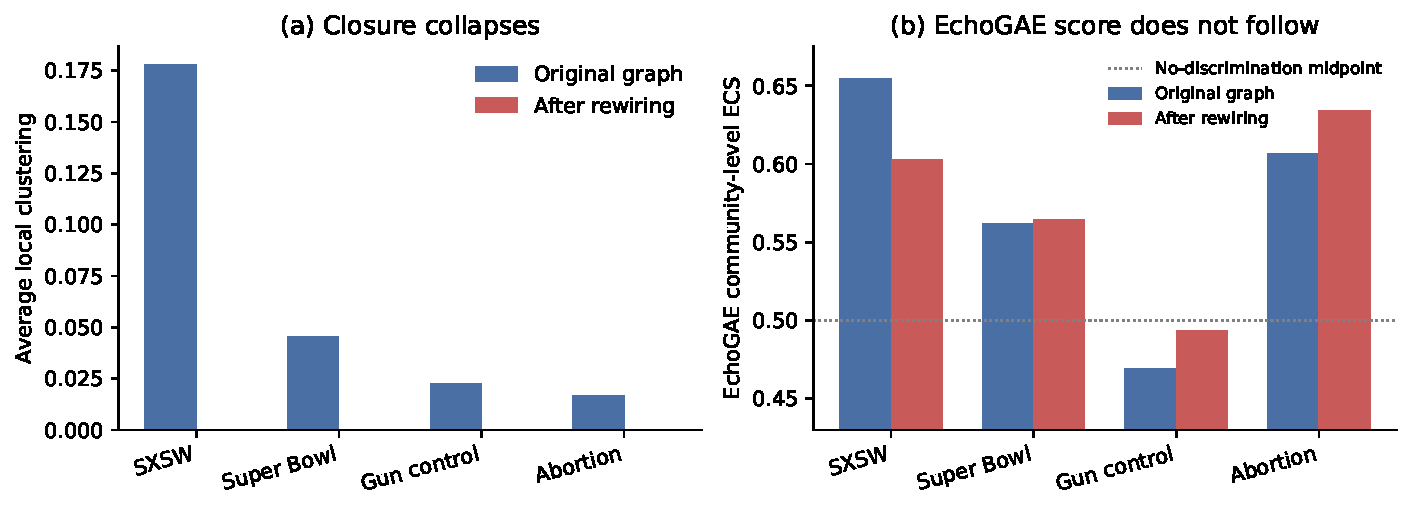
\includegraphics[width=\linewidth]{figures/rewire_v2_side_by_side.pdf}
\caption{Rewiring on EchoGAE's four datasets under the paper's exact
Louvain pipeline. (a) Average local clustering collapses on every
topic. (b) EchoGAE's community-level ECS moves by
$0.003$--$0.052$ against a $0.5$ no-discrimination midpoint; the
$0.5$ line is drawn for reference. A closure-tracking estimator
would show a large drop in Panel (b) tracking the collapse in Panel
(a); EchoGAE does not.}\label{fig:rewire}
\end{figure}

Figure~\ref{fig:rewire} puts the closure signal and the score
side by side. Panel (a) shows clustering collapsing on every
topic; Panel (b) shows the score staying inside a $0.08$ band.

Cross-referencing Table~\ref{tab:rewire} against
Table~\ref{tab:wl-tv} sharpens the reading. On three topics
(gun, abortion, SXSW) the rewiring produces a depth-$2$ $1$-WL
TV of $0.69$--$0.79$, which a two-layer encoder can detect; the
$\Delta$ECS on those topics is $0.025$, $0.027$, $-0.052$. On
Super Bowl the depth-$2$ TV is $0.10$ and $\Delta$ECS is
$0.003$; the two agree. Super Bowl's near-invariance is
consistent with the rewiring producing little depth-$2$ signal;
the other three topics' near-invariance is not.

The ratio $|\Delta$ECS$| / d_{TV}(h_2)$ in
Table~\ref{tab:wl-tv} makes the compression quantitative.
Proposition~\ref{prop:rewire-bound} bounds this ratio by the
range of the estimator's output ($1$ for ECS $\in [0, 1]$); the
observed values sit between $0.031$ and $0.066$. EchoGAE's
readout passes roughly $3$--$7\%$ of the depth-$2$ WL variation
through to the score. A closure-tracking estimator running on the
same graphs would pass a much larger fraction, because closure
destruction is one of the depth-$2$ changes the rewiring
produces.

\subsection{What a CSS reader should conclude}\label{sec:reading}

\emph{Do not treat a published ECS as a numerical polarisation
measurement.} Across $10$ seeds under EchoGAE's own pipeline with
the SBERT model pinned, three of four published Twitter numbers
sit $2.8$ to $9.3$ standard deviations from our reproduction; the
paper's ranking of the four topics is not preserved. A published
ECS value is not reproducible to the precision at which
cross-topic differences of $0.1$--$0.2$ are argued.

\emph{Do not read cross-topic ECS differences as evidence of
differential polarisation.} On the paper's own numbers the
polarising-versus-non-polarising gap is $0.195$ with no reported
variability. On our reproduction the four means are $\{0.43,
0.64, 0.60, 0.64\}$; the two groups do not separate. A
permutation test on matched-size random block assignments
gives a null gap of $-0.127 \pm 0.023$ (non-polarising
higher), against which the paper's $+0.195$ sits on the
opposite side of the null mean at $p = 0.002$.

\emph{Do not read an ECS number as a measurement of closure
structure.} A rewiring that removes almost all triadic closure
while preserving degrees and Louvain-block edge counts moves the
community-level ECS by $0.003$--$0.052$ on $[0, 1]$
(Figure~\ref{fig:rewire}). A closure-tracking score would drop in
step; EchoGAE does not.

\emph{Expect much of the score to be graph-blind.} On the two
topics with more than two communities, community size alone
accounts for a raw Pearson $r^2$ of $0.49$ (Super Bowl) and
$0.72$ (SXSW); pooled across topics after within-topic rank
transformation, $r^2 = 0.20$ with $95\%$ CI $[0.01, 0.61]$. The
n is small and the interval is wide; the direction is what
depth-$1$ ego-net factorisation
(Proposition~\ref{prop:egonet}) predicts.

\subsection{A second target: InfoVGAE}\label{sec:infovgae}

InfoVGAE \citep{Li22InfoVGAE} is a variational graph
auto-encoder with a GCN encoder, a low-dimensional non-negative
latent, a PID-controlled KL weight, and a total-correlation
discriminator, trained on a bipartite user-claim graph (a claim
is a tweet cascade) with identity input features. Its paper
evaluates it by $2$-means clustering of the user latent against
stance labels and reports precision, recall, F1, and purity
(its Table~1) from single runs at seed $0$.

\emph{In its own setting.} We run the released pipeline on its
two Twitter datasets under its own configuration
($3$-dimensional latent; $80$ epochs on Election, $118$ on
Eurovision; the release's preprocessing thresholds): Election
($502$ users, $4{,}159$ claims, $6{,}877$ user-claim edges,
$145$ labelled users) and Eurovision ($483$ users, $1{,}054$
claims, $2{,}512$ edges, $480$ labelled users). Two patches
were needed: current \texttt{torch} rejects cross-entropy
targets outside $[0, 1]$, so user-claim counts above $1$ ($76$
and $122$ entries) are clipped, and the seed is set after the
config is applied, because the config file overwrites it with
$0$. At seed $0$ the patched pipeline returns user F1 $0.882$ on
Election, the paper's $0.8819$. Across seeds $42$--$51$
(Table~\ref{tab:infovgae-native}) the user F1 is
$0.731 \pm 0.100$ on Election, range $[0.638, 0.880]$, and
$0.623 \pm 0.140$ on Eurovision, range $[0.447, 0.854]$;
purity is $0.672 \pm 0.154$ and $0.760 \pm 0.086$ against the
published $0.860$ and $0.884$. The published F1 values sit
$1.5\sigma$ and $1.7\sigma$ above the seed means; on Election
two of ten seeds reach the published value, on Eurovision none.
A control with counts clipped but no rewiring is within $0.05$
of the original on every statistic, so the patch is not the
source of the spread.

\begin{table}[t]
\centering
\small
\setlength{\tabcolsep}{3pt}
\begin{tabular}{llrrr}
\toprule
& & Paper & Original & Rewired \\
\midrule
\multirow{2}{*}{Election}
& user F1 & $0.882$ & $0.731 \pm 0.100$ & $0.688 \pm 0.048$ \\
& purity  & $0.860$ & $0.672 \pm 0.154$ & $0.615 \pm 0.074$ \\
\multirow{2}{*}{Eurovision}
& user F1 & $0.866$ & $0.623 \pm 0.140$ & $0.928 \pm 0.027$ \\
& purity  & $0.884$ & $0.760 \pm 0.086$ & $0.958 \pm 0.017$ \\
\bottomrule
\end{tabular}
\caption{InfoVGAE in its own setting, $10$ seeds. Paper: the
single-run values in \citet{Li22InfoVGAE}, Table~1. Original:
the released pipeline. Rewired: the user-claim graph after a
bipartite swap that preserves every degree and every node's
neighbourhood label composition and randomises the rest;
butterfly counts fall from $6{,}650$ to $3{,}200$--$3{,}900$
(Election) and from $4{,}478$ to $1{,}800$--$2{,}200$
(Eurovision). F1 ranges: Election $[0.638, 0.880]$ original,
$[0.643, 0.780]$ rewired; Eurovision $[0.447, 0.854]$ original,
$[0.887, 0.957]$ rewired.}\label{tab:infovgae-native}
\end{table}

\emph{Response.} For each seed we apply a bipartite double-edge
swap to the binarised user-claim graph, accepting a swap only
when the two users carry the same stance label and the two
claims carry the same label. Every user's degree, every claim's
degree, and the label composition of every node's
neighbourhood are preserved exactly; which user posted which
claim is otherwise randomised. Ten accepted swaps per edge
roughly halve the butterfly count (two users sharing two
claims, the bipartite closure statistic). On Election the
rewired user F1 is $0.688 \pm 0.048$, a change of $-0.04$; on
Eurovision it is $0.928 \pm 0.027$, a change of $+0.31$, with
all ten seeds above the published value. The sign difference
tracks label coverage: Eurovision has $99\%$ of its claims
labelled and $99\%$ of its users, so almost every edge is
constrained to preserve the block pair, and the rewire is a
within-block permutation. Election has $2\%$ of its claims
labelled and $29\%$ of its users, so most edges are free, and
the rewire is closer to a full permutation of the graph. On
the label-constrained dataset the model separates the label
blocks of the randomised graph better, and far more
consistently, than the real one. The release
ships a third Twitter dataset, built from TIMME's politician
accounts ($430$ users, $2{,}437$ claims, $17{,}526$ edges, all
users labelled), for which the paper reports no number; there
the ten-seed user F1 is $0.937 \pm 0.057$, range
$[0.793, 0.974]$, and the rewired graph again scores higher
and tighter, $0.981 \pm 0.021$.

\emph{Reading.} InfoVGAE takes identity input features, so its
latent is a function of graph structure alone. The two datasets
agree on a seed-level spread of $0.10$--$0.14$ in a number the
paper reports once, with the published value at the top of the
seed distribution. They disagree on the direction of the
response to the same perturbation. A score that a seed change
moves by $0.2$--$0.4$, and that a label-composition-preserving
rewiring can raise above its published value, is not a stable
measurement of stance structure in the real graph; on
Eurovision, the real graph's structure beyond label composition
works against the model.

\emph{On EchoGAE's graphs.} A secondary adaptation running
InfoVGAE on EchoGAE's user-user topics with a two-column
feature matrix and a $2$-dimensional latent is deferred to
Appendix~\ref{app:infovgae-adapt}; it agrees on the training
instability, adds no new finding.

\subsection{A third target: TIMME}\label{sec:timme}

TIMME \citep{XiaoTIMME2020} is a supervised estimator: a
multi-relational GCN trained end to end to predict the
Democrat/Republican ideology label of a Twitter account from
five directed relations (retweet, mention, friend, reply,
favorite) and per-user GloVe features. We run two of its
released datasets: PureP ($583$ accounts, $122{,}347$ directed
relation records, $581$ labels after removing independents and
unmatched ids), the smallest and TIMME's default; and P50
($5{,}435$ accounts, $1{,}593{,}721$ directed relation records,
$756$ labels), the next size up. Both go through TIMME's own
\texttt{main.py} on the default \texttt{Classification} task,
hyperparameters unchanged from the release.

\emph{Reproducibility.} Across $10$ seeds
$s \in \{42, \ldots, 51\}$ threaded through
\texttt{numpy}, Python \texttt{random}, and \texttt{torch},
TIMME's test accuracy on PureP is $0.976 \pm 0.024$, range
$[0.930, 1.000]$; on P50 it is $0.927 \pm 0.056$, range
$[0.773, 0.960]$. The test sets hold $57$ and $75$ accounts,
so one misclassified account moves accuracy by $1.8$ and
$1.3$ pp. TIMME's Table~2 reports $1.000$ on PureP and
$0.973$ on P50 for this single-task classifier, single runs
with no variance. Both published values sit within one
across-seed standard deviation of our mean and at the upper
end of the seed distribution: $3$ of $10$ PureP seeds reach
$1.000$; no P50 seed reaches $0.973$, and one falls to
$0.773$. A supervised model whose release reports a single
run has a seed-level spread of $2$--$6$ pp on these datasets.

\emph{Graph-blind ceiling.} A logistic regression on the same
\texttt{tweets\_average} GloVe features TIMME accepts as node
inputs, no adjacency, no message passing, reaches
$0.891 \pm 0.023$ on PureP and $0.883 \pm 0.020$ on P50 across
the same $10$ seeds under the same $80/10/10$ split (which
Python \texttt{random} fixes from the seed). The graph adds
$8.5$ pp on PureP and $4.4$ pp on P50 over a node-feature
classifier; the graph contributes, but on both datasets most
of the headline accuracy is available without it.

\emph{Response.} TIMME reads each relation as a table of
(source, target, count) records and binarises it into a
directed adjacency. For each seed we shuffle the records of
each relation by directed double-edge swaps
$(a, b), (c, d) \to (a, d), (c, b)$, accepting a swap only
when the two records carry the same label-block pair (from
$\{\mathrm{D}, \mathrm{R}, \mathrm{U}\}^2$, U for unlabelled)
and neither target record already exists. Each swap preserves,
for every account, its number of source and target records in
the relation and the label-block composition of its record
neighbourhood. On PureP the accepted swaps per relation and
seed are $33{,}186$ (retweet), $52{,}590$ (mention),
$29{,}536$ (friend), $22{,}369$ (favorite), and about
$1{,}600$ on reply, the sparsest relation ($1{,}451$ records),
which stops at the $60$ s wall-clock cap. On P50 the cap is
$200{,}000$ swaps per relation; eight of ten seeds reach it on
all five relations, and the other two stop earlier under the
wall-clock cap (minimum $33{,}936$ on reply at one seed). The
shuffled tables are then run through TIMME's own
\texttt{main.py} at the same seed with a matching
\texttt{PYTHONHASHSEED} (TIMME's id-to-row map consumes Python
set iteration order, which otherwise varies across processes
at fixed model seeds).

\begin{table}[t]
\centering
\small
\setlength{\tabcolsep}{3pt}
\begin{tabular}{llrrr}
\toprule
& Relation & Unique edges & Triangles & $|\Delta f_{\mathrm{D}}|$ \\
\midrule
\multirow{5}{*}{\rotatebox{90}{PureP}}
& retweet  & $19.3\mathrm{k} \to 35.4\mathrm{k}$ & $0.18\mathrm{M} \to 0.79\mathrm{M}$ & $0.036$ \\
& mention  & $27.1\mathrm{k} \to 57.1\mathrm{k}$ & $0.25\mathrm{M} \to 1.79\mathrm{M}$ & $0.057$ \\
& friend   & $59.1\mathrm{k} \to 59.1\mathrm{k}$ & $1.59\mathrm{M} \to 1.86\mathrm{M}$ & $0.000$ \\
& reply    & $925 \to 1081$ & $93 \to 189$ & $0.011$ \\
& favorite & $14.0\mathrm{k} \to 26.9\mathrm{k}$ & $0.08\mathrm{M} \to 0.48\mathrm{M}$ & $0.027$ \\
\midrule
\multirow{5}{*}{\rotatebox{90}{P50}}
& retweet  & $308\mathrm{k} \to 543\mathrm{k}$ & $6.3\mathrm{M} \to 30.1\mathrm{M}$ & $0.011$ \\
& mention  & $351\mathrm{k} \to 593\mathrm{k}$ & $6.9\mathrm{M} \to 31.3\mathrm{M}$ & $0.018$ \\
& friend   & $529\mathrm{k} \to 529\mathrm{k}$ & $14.9\mathrm{M} \to 14.6\mathrm{M}$ & $0.000$ \\
& reply    & $93\mathrm{k} \to 184\mathrm{k}$ & $0.14\mathrm{M} \to 2.19\mathrm{M}$ & $0.006$ \\
& favorite & $300\mathrm{k} \to 538\mathrm{k}$ & $4.2\mathrm{M} \to 25.0\mathrm{M}$ & $0.006$ \\
\bottomrule
\end{tabular}
\caption{What the TIMME shuffle changes and what it keeps, seed
$42$. Unique edges: distinct directed pairs in the binarised
relation TIMME consumes. Triangles: on the undirected simple
projection of the relation. $|\Delta f_{\mathrm{D}}|$: mean
absolute change, over labelled accounts, in the Democrat
fraction of their labelled out-neighbours. On the friend
relation every record has count $1$, so the shuffle preserves
binarised degrees and neighbourhood label composition exactly;
on the four weighted relations, parallel records spread to new
pairs and the binarised graph gains $70$--$110\%$ more edges,
while neighbourhood label composition moves by at most $0.06$
on average.}\label{tab:timme-closure}
\end{table}

Table~\ref{tab:timme-closure} records how far the binarised
graph moves. The shuffle is not closure-removing in the sense
of Section~\ref{sec:exp-rewire}: on the four weighted
relations, parallel records disperse to new pairs, unique
directed edges rise by $70$--$110\%$, and triangle counts
rise by a factor of $2$ to $6$; average local clustering on
the union graph goes from $0.61$ to $0.72$ on PureP and from
$0.43$ to $0.50$ on P50. Neighbour identity is randomised
subject to the label-block constraint. What survives is each
account's neighbourhood label composition, exactly on the
friend relation (the largest, all counts $1$) and to within a
mean absolute change of $0.006$--$0.057$ in the Democrat
fraction on the others.

On PureP the shuffled test accuracy is $0.970 \pm 0.014$; the
delta is $-0.005 \pm 0.020$, range $[-0.035, +0.035]$, sign
inconsistent across seeds. On P50 the shuffled test accuracy
is $0.968 \pm 0.025$ and the delta is $+0.041 \pm 0.066$,
range $[-0.013, +0.213]$: at the seed where TIMME's original
accuracy falls to $0.773$, the shuffled graph trains to
$0.987$; on the other nine seeds the delta lies within one
across-seed standard deviation of the original. The mild
positive mean on P50 has a plausible mechanism in the table:
the binarised shuffled graph is denser, so each account
averages over more labelled neighbours of the same
composition. On both datasets the delta is inside the seed
noise floor while the graph has changed by every measure in
Table~\ref{tab:timme-closure} except neighbourhood label
composition.

\emph{Closure removal.} The shuffle raises closure; the
EchoGAE null lowers it. To run that null on TIMME we binarise
each relation first (which is what TIMME sees) and apply the
same directed swap with the triangle-destroying acceptance
rule of Section~\ref{sec:exp-rewire}, with a budget of ten
accepted swaps per edge. Binarised in-degree, out-degree, and
neighbourhood label composition are then preserved exactly, so
the depth-$1$ colour histogram under label-block initial
colours is unchanged. On PureP the swaps cut triangle counts
by $91$--$97\%$ on retweet, mention, and favorite
($182\mathrm{k} \to 9$--$10\mathrm{k}$, $248\mathrm{k} \to
22$--$24\mathrm{k}$, $80\mathrm{k} \to 2\mathrm{k}$) and by
$27$--$40\%$ on the dense friend relation, where the
acceptance rate is low; reply has $93$ triangles to begin
with. TIMME's test accuracy on the closure-removed PureP is
$0.944 \pm 0.058$; the delta is $-0.032 \pm 0.046$, range
$[-0.123, +0.018]$. Seven of ten seeds move by at most one
test account; three seeds lose $4$--$7$ of the $57$. On P50
the same procedure (five seeds; $600$ s wall-clock cap per
relation) cuts triangles on the three sparse relations by
$70$--$95\%$ and leaves the friend relation at
$67$--$91\%$ of its original triangle count. The test
accuracy is $0.973 \pm 0.016$; the delta is
$+0.029 \pm 0.015$, range $[+0.013, +0.053]$, positive on all
five seeds. The two datasets bracket the finding: on the
smaller graph the two-layer model does see some of the
depth-$2$ change, on some seeds; on the larger graph the
change tightens the accuracy rather than degrading it. In
neither case is the mean move as large as the $4$--$8$ pp the
graph adds over the graph-blind baseline.

\emph{Reading.} TIMME's authors do not present it as a
closure measurement, and neither test asks it to be one. The
two tests together isolate what in the graph the $4$--$8$ pp
increment over the graph-blind baseline depends on. Under the
shuffle, triangle density, unique-edge density, and the
identity of an account's neighbours change by large factors
without moving the accuracy. Under closure removal, with
degrees and neighbourhood label composition held fixed
exactly, the accuracy moves by $3$ pp in either direction (
$-3$ pp on PureP, $+3$ pp on P50), and on most PureP seeds by
$0$--$1$ test accounts. The label composition of the
neighbourhood is the quantity both tests hold fixed, and it is
the homophily-shaped invariant Section~\ref{sec:framework}
places inside the MPNN class. On P50, with ten times PureP's
vertex count, the shuffle delta is again inside the seed noise
floor and the direction moves from inconsistent to mildly
positive, so the PureP result is not a small-graph artefact. A
downstream reading of a TIMME score that attributes it to who
an account interacts with, or mainly to closure among its
contacts, is not supported by the model's response on either
dataset; a reading as node features plus label homophily, with
a few points of closure-sensitive residue on some seeds, is.

\subsection{A Reddit supplement}\label{sec:reddit}

Intersecting the SNAP soc-RedditHyperlinks release
\citep{KumarRedditHyperlinks2018} (subreddit-to-subreddit
hyperlinks from post bodies, multiplicity $\ge 3$) with the
Waller-Anderson community set \citep{WallerAnderson2021} and
taking the largest connected component gives $3{,}662$ subreddits
and $10{,}750$ edges. Every vertex carries the Waller-Anderson
partisan-axis score. We run the same protocol as on the Twitter
graphs, across $10$ seeds.

\emph{Reproducibility.} The community-level ECS is $0.623 \pm
0.004$; the graph-blind $R^2$ (ridge on the seven per-community
features) is $0.28 \pm 0.01$. The graph-blind fraction is
larger than on the Twitter graphs (Table~\ref{tab:blind}),
consistent with a graph on which first-order neighbourhood
structure carries most of the score.

\emph{Response.} The rewiring removes all clustering
($0.291 \to 0.000$, $26{,}413$ triangles) while keeping the graph
connected. To separate rewire-instance variance from
training-seed variance we run $5$ independent rewires at $5$
training seeds each. All five rewires give a negative mean
delta ($-0.011$ to $-0.026$, mean $-0.017 \pm 0.005$
between-rewire); the within-rewire training variance is
$\sqrt{2.8 \times 10^{-4}} = 0.017$, nine times the
between-rewire component. The response direction is stable;
its magnitude sits at one training-seed standard deviation.

\subsection{Direct estimators on the same graphs}\label{sec:direct}

The recommendation in Section~\ref{sec:recs} is to reach for a
direct estimator when the target is closure- or spectral-shaped
and for a direct assortativity or modularity computation when
the target is homophily-shaped. Table~\ref{tab:direct} gives
those numbers on all seven audit graphs. They take under a
minute to compute per dataset, are deterministic single-graph
functionals, and carry no seed variance.

\begin{table}[t]
\centering
\small
\setlength{\tabcolsep}{4pt}
\begin{tabular}{lrrrl}
\toprule
Dataset & $\bar c$ & mod. & assortativity (95\% CI) & RWC \\
\midrule
Gun         & $0.02$ & $0.96$ & $+0.67\ [+0.51, +0.84]$ & $0.46$ \\
Abortion    & $0.02$ & $0.95$ & $+0.44\ [+0.35, +0.52]$ & $0.31$ \\
Super Bowl  & $0.05$ & $0.95$ & $+0.54\ [-0.05, +0.89]$ & $0.59$ \\
SXSW        & $0.18$ & $0.96$ & $-0.03\ [-0.19, +0.47]$ & --- \\
Reddit      & $0.31$ & $0.62$ & $+0.19\ [+0.15, +0.25]$ & $0.09$ \\
PureP       & $0.61$ & $0.27$ & $+0.52\ [+0.49, +0.55]$ & $0.06$ \\
P50         & $0.43$ & $0.21$ & $+0.49\ [+0.47, +0.52]$ & $0.04$ \\
Polblogs    & $0.32$ & $0.43$ & $+0.81\ [+0.78, +0.84]$ & $0.61$ \\
\bottomrule
\end{tabular}
\caption{Direct polarisation statistics on the seven audit
datasets: average local clustering, modularity of the Louvain
partition at the audit's resolution and seed, Newman signed
attribute assortativity on the label sign (with $95\%$ CI
from $500$ bootstrap resamples of the labelled subset), and
Garimella-style RWC on the two-side split ($k = 20$
authorities, $500$ walks per side, seed $42$). Bootstrap CIs
on Super Bowl and SXSW are wide because those topics have
only $\sim\!200$ labelled vertices. SXSW's RWC has too few
labelled vertices in each partition to
stabilise.}\label{tab:direct}
\end{table}

Two readings.
\emph{Polarising vs non-polarising}, the four-topic claim
EchoGAE's Table~2 is used for. Assortativity gives $0.55$ mean
across the two polarising topics and $0.26$ across the two
non-polarising, a $0.29$ gap. Gun's $95\%$ CI $[0.51, 0.84]$
does not overlap SXSW's mean $-0.03$; abortion's $[0.35, 0.52]$
does not overlap SXSW's either; Super Bowl's CI is wide
($[-0.05, 0.89]$) because it has only $195$ labelled
vertices. The paper's claim of polarising-versus-non-polarising
separation survives on three of the four cross-topic
comparisons, without training an encoder or picking a seed.
\emph{Reddit and TIMME}. Reddit's assortativity is $0.19$ at
the partisan-axis sign; TIMME's PureP and P50 land at $0.52$
and $0.49$ against a supervised classifier reaching $0.976$ and
$0.927$. On both, the MPNN score's increment over the direct
statistic is the quantity worth reporting, and a paper that
cites a TIMME accuracy alongside a Newman assortativity makes
that increment visible.

\emph{Convergent validity.} What does the reproduced ECS
correlate with across the four EchoGAE topics? Its ranking
(gun $<$ abortion $\approx$ sxsw $\approx$ super bowl) has
Spearman $-1.00$ with the assortativity ranking (gun highest,
sxsw lowest) and $+0.40$ with the clustering ranking. ECS
aligns with neither reading, and where it aligns weakly, with
clustering.

\emph{A benchmark point.} Table~\ref{tab:direct} also
includes the Adamic-Glance political-blogs graph
\citep{AdamicGlance2005}, the canonical polarisation benchmark
in the CSS literature, on which no audited model is
trained or claimed to work; direct estimators put it at
assortativity $0.81\ [0.78, 0.84]$ and RWC $0.61$, values
consistent with two decades of reading of that graph as
sharply polarised. On the eight-dataset table the direct
statistics order the graphs as any CSS reader familiar with
this literature would predict; the seeded MPNN scores do not.

\emph{A compliant report.} On our Reddit subgraph, the
polarisation summary would read: $3{,}662$ subreddits,
$10{,}750$ edges, Waller-Anderson partisan-axis sign as the
label; edge-homophily $0.63$, Newman assortativity
$+0.19\ [+0.15, +0.25]$ ($500$-bootstrap CI), modularity of
Louvain partition $0.62$, average local clustering $0.31$,
RWC on the two-side split $0.09$. Six deterministic numbers
against a graph description, no seeds, no training. That is
what the CSS reader looking at an ECS number wants; direct
statistics deliver it.

\subsection{A closure-sensitive baseline}\label{sec:gsn}

On SXSW, the topic with the largest clustering
($0.178$, roughly ten times the other three) and largest
$|\Delta\mathrm{ECS}|$ under the rewire, an ECS distance
computed on the raw two-feature vector (triangle count,
degree) moves from $0.407$ to $0.351$ under the same rewire
($-0.056$); EchoGAE on SXSW moves by $-0.052$, same direction,
comparable magnitude. Feeding the triangle-count features
through the EchoGAE encoder gives $\Delta = +0.049$, opposite
in sign: the encoder absorbs the lifted colouring into its own
fixed point. On the one graph with substantial closure the
score does move in the closure-consistent direction; on the
three low-closure graphs there is little closure to move. A
subgraph-count MPNN \citep{Bouritsas2022} that injects
subgraph counts into the update would give a sharper
separation; we do not implement one.

\section{Related work}\label{sec:related}

\paragraph{GNN expressiveness.} Message-passing GNNs
\citep{GilmerNeuralMessagePassing2017} are $1$-WL-bounded
\citep{MorrisWL2019, XuGIN2019}; universal approximation of
$1$-WL invariants was established by \citet{ChenVillar2019}
and \citet{AzizianLelarge2021}. Higher-order $k$-WL and
subgraph-count architectures \citep{Bouritsas2022} escape
the bound. Graphon-limit theory \citep{KerivenPeyre2020,
RuizChamonRibeiro2021} gives universality in the dense
limit; our impossibility is in the sparse regime interaction
graphs inhabit.

\paragraph{Polarisation measurement.} Homophily and
modularity are long-standing \citep{Newman2003, Newman2004,
AdamicGlance2005, ConoverPolBlogs2011}; structural measures
include random walk controversy \citep{Garimella18},
spectral GED \citep{Hohmann2016, HohmannGED2023}, subreddit
community embeddings \citep{WallerAnderson2021}, and
Bayesian ideal-point models \citep{Barbera2015}. None of
this literature connects the choice of measure to the
expressiveness class of the estimator.

\paragraph{GNN polarisation estimators.} EchoGAE
\citep{Alatawi23EchoGAE}, InfoVGAE \citep{Li22InfoVGAE}, and
TIMME \citep{XiaoTIMME2020} are the MPNN estimators in scope
of Theorem~\ref{thm:dichotomy}. TIMME differs in being
supervised; its audit correspondingly reports classification
accuracy rather than an unsupervised score.

\paragraph{Null-model rewiring.} Degree-preserving rewiring goes
back to \citet{MolloyReed1995, Newman2001}. The degree-corrected
SBM is \citet{Karrer2011StochasticBlock}. The seed-sensitivity of GNN
predictions has itself been documented outside our audit
\citep{ErricaFair2020}. Adversarial GNN
perturbations \citep{Jin2020, Zugner2018} share the mechanism but
differ in objective: adversarial robustness maximises output
change under worst-case edge perturbations, whereas the rewiring
here is constrained to preserve $1$-WL statistics computable at
depth $1$. Joint degree- and block-preserving rewiring is a
common configuration-model variant in network science; its use
as an identifiability test for GNN estimators is where this
paper adds.

\section{Recommendations for practitioners}\label{sec:recs}

The recommendations below extend two long-running conversations
in computational social science: the reproducibility discussion
initiated in this field by \citet{LazerObstacles2020} and
formalised into a tier system by \citet{Schoch2024Reproducibility},
and the construct-validity discussion of
\citet{JacobsWallach2021} on the mismatch between theoretical
polarisation constructs and their operationalisations. The
practices below apply the general principles those papers
articulate to the specific case of GNN-based polarisation
scores. For a broader CSS-methodology framing see
\citet{Salganik2018BitByBit}.

\paragraph{Where this matters in practice.} The estimators are
already in downstream use. \citet{Riedl2024GermanElection}
apply Alatawi's ECS to a COVID-19 Twitter dataset and read
values above $0.5$ as evidence of a strong echo-chamber
effect; our rewire moves the score by up to $0.052$ on the
same $[0, 1]$ range, so a $0.05$-margin threshold sits inside
the identifiability floor of the estimator on our data.
\citet{Ghafouri2024Transformer} extend the ECS with a
transformer-based user representation on Twitter topics and
inherit the same MPNN-in-scope readout.
\citet{Sun2023Decoding} use InfoVGAE as a baseline whose
$0.10$--$0.14$ seed-level F1 spread (Section~\ref{sec:infovgae})
is uncertainty downstream pipelines inherit.

\paragraph{When using EchoGAE or InfoVGAE.} Do not report the
graph-level ECS or the InfoVGAE latent score as a polarisation
measurement. Use either at most as a homophily proxy on the
labelled subset. Pin the Sentence-BERT model to a HuggingFace
revision, run at least $10$ seeds, and report the across-seed
standard deviation; InfoVGAE's published evaluation is a single
run at seed $0$, and the ten-seed spread in its own setting is
$0.10$--$0.14$ in F1. Run the degree- and community-preserving
rewiring test and report the rewire delta next to the score; a
delta smaller than a closure-tracking estimator would give is
grounds to downgrade any claim that the score measures
echo-chamber structure.

\paragraph{When using TIMME or a similar supervised MPNN
ideology estimator.} The
\citet{Schoch2024Reproducibility, JacobsWallach2021} concerns
apply as they do to unsupervised estimators. Report
across-seed variance: the release reports single runs; the
seed-level spread is $2$--$6$ pp on TIMME's datasets. Report
the graph-blind logistic regression on the same node features
next to the classification accuracy; on PureP and P50 it
reaches $0.891$ and $0.883$ against TIMME's $0.976$ and
$0.927$, so the graph adds $4$--$8$ pp. Report the deltas
under the two rewires from Section~\ref{sec:timme}: the
label-composition-preserving shuffle
($-0.005 \pm 0.020$, $+0.041 \pm 0.066$) and the
closure-removing rewire ($-0.03 \pm 0.05$, $+0.03 \pm 0.02$).
Together they separate ``the model uses neighbourhood label
composition'' from ``the model uses who an account interacts
with, or closure among its contacts.'' Fix
\texttt{PYTHONHASHSEED} in addition to the model seeds:
TIMME's \texttt{utils.py} builds its account-to-row index by
iterating a \texttt{set()} of ids, so cross-process results
differ at identical model seeds unless the hash seed is also
pinned, a form of the reproducibility gap
\citet{LazerObstacles2020} name as characteristic of CSS
pipelines.

\paragraph{Reading and choosing.} Ask what structural
quantity the paper commits to. If it is homophily or
modularity of a fixed partition, an MPNN can track it and the
question is one of evaluation; if closure (triadic density,
clustering, community insularity) or spectral (GED, boundary
conductance), the architecture cannot compute it, and the
score's agreement with the target is evidence about a $1$-WL
invariant proxy. For the homophily-shaped case, a direct
assortativity computation is simpler and reproduces exactly;
for the closure or spectral case, use a direct statistic
(Table~\ref{tab:direct}) or an architecture outside the
message-passing class (subgraph-count GNNs, higher-order
Weisfeiler-Leman, Bayesian ideal-point models
\citep{Barbera2015}). The audit itself is cheap: the $10$-seed
EchoGAE reproduction on the four Twitter graphs takes about
an hour of laptop CPU, the rewiring pass about the same.

\section{Discussion}\label{sec:discussion}

The audit outcomes for all three estimators are consistent
with the bound in Section~\ref{sec:framework}: an MPNN
estimator's output is a functional of the graph's $1$-WL
colour histogram, and closure-based polarisation measures lie
outside that class. Weak response to closure destruction
(EchoGAE, InfoVGAE) and invariance under a shuffle that
preserves neighbourhood label composition (TIMME) are what
the bound permits, not what it predicts: at a depth-$2$ WL TV
of $0.69$--$0.79$ under the EchoGAE rewiring, the bound
allows any $|\Delta \mathrm{ECS}| \in [0, 1]$, so the observed
$0.003$--$0.052$ says something empirical about the trained
readout compressing that variation, not something implied by
the architecture class. The finding on TIMME's shuffle
similarly identifies which invariant the accuracy depends on
(neighbourhood label composition), which is inside the class,
without ruling out that a different trained readout would use
more. Non-reproduction
(EchoGAE) is a pipeline finding the bound does not speak to;
training-run instability (InfoVGAE, in its own setting and in
the adaptation) is a separate variational pathology (posterior
collapse, PID-controlled KL with disagreeing seeds) that the
bound does not imply either. Both
push in the same direction: the score is not a stable graph
functional.

\paragraph{Limitations.} The audit covers three estimators on
ten datasets (EchoGAE's four Twitter graphs, one Reddit
graph, TIMME's PureP and P50, InfoVGAE's Election and
Eurovision, and the Adamic-Glance political-blogs graph
\citep{AdamicGlance2005} as an external benchmark). TIMME is audited on its own released datasets only,
not on the four EchoGAE topics; re-training TIMME on the
EchoGAE topics would require ideology labels for their
accounts, which are not part of the released EchoGAE datasets.
The two larger TIMME datasets (P\_20\_50 and P\_all) are not
included; P50 has ten times PureP's vertex count and gives the
same result on all three properties. The closure-removing
rewire of TIMME's relations leaves the friend relation
with $60$--$73\%$ of its triangles on PureP and $67$--$91\%$
on P50; triangle-destroying swaps are rarely accepted on the
densest relation, and its closure test is partial. On P50 the
closure rewire is run at five seeds under a $600$ s per-relation
cap, not ten seeds under a $60$ s cap as on PureP. The native-setting InfoVGAE runs use ten seeds and the release's
own datasets and configuration; the adaptation to EchoGAE's
user-user graphs (Appendix~\ref{app:infovgae-adapt}) also uses
ten seeds on three of four topics and defers gun. The ensemble MSE lower bound
(Appendix~\ref{app:entangle}) is on structurally uniform
ensembles (monochromatic triangles or $6$-cycles) and does not
extend to matched-moment planted-partition models
(Appendix~\ref{app:ppm}). The audit identifies what functional
an estimator does not compute; it does not by itself explain
why an MPNN score correlates, when it does, with human
polarisation labels; that would require a separate step
connecting the estimator's implicit functional to the label
distribution.

\paragraph{Ethics.} The audit uses public datasets under their
original licences and does not identify individual accounts
beyond what those datasets already publish. Nothing in the paper
depends on the identities of individual users.

\section*{Acknowledgements}

Anonymised for review. Generative AI tools assisted with LaTeX
and Python scaffolding; all mathematical content, experimental
design, and conclusions are the authors'.

\bibliography{references}

\section*{Paper Checklist}
\begin{enumerate}
\item For most authors\ldots
  \begin{enumerate}
  \item Would answering this research question advance science
    without violating social contracts, such as violating privacy
    norms, perpetuating unfair profiling, exacerbating the
    socio-economic divide, or implying disrespect to societies or
    cultures? \textbf{Yes.} The paper audits published estimators
    on public datasets and reports what they compute; it does not
    identify individuals.
  \item Do your main claims in the abstract and introduction
    accurately reflect the paper's contributions and scope?
    \textbf{Yes.}
  \item Do you clarify how the proposed methodological approach is
    appropriate for the claims made? \textbf{Yes.} The
    audit design follows from
    Proposition~\ref{prop:egonet}.
  \item Do you clarify what are possible artifacts in the data
    used, given population-specific distributions? \textbf{Yes.}
    Section~\ref{sec:exp-repro} pins the Sentence-BERT model to a
    specific HuggingFace revision to eliminate weight drift, and
    discusses the AllSides rating drift and networkx-vs.-python-louvain
    variance as the remaining gap sources.
  \item Did you describe the limitations of your work?
    \textbf{Yes.} See Section~\ref{sec:discussion}.
  \item Did you discuss any potential negative societal impacts
    of your work? \textbf{Yes.} An audit that pushes back on
    polarisation-detection methodology could be misread as
    denying that echo chambers exist; the paper is explicit that
    it is about what MPNN estimators measure, not whether echo
    chambers exist.
  \item Did you discuss any potential misuse of your work?
    \textbf{Not applicable.} The audit procedure is a
    reproducibility check.
  \item Did you describe steps taken to prevent or mitigate
    potential negative outcomes of the research, such as data
    and model documentation, data anonymization, responsible
    release, access control, and the reproducibility of
    findings? \textbf{Yes.} All code and preprocessing are
    released with the submission.
  \item Have you read the ethics review guidelines and ensured
    that your paper conforms to them? \textbf{Yes.}
  \end{enumerate}
\item Does this paper make theoretical contributions? \textbf{Yes.}
  \begin{enumerate}
  \item All assumptions and restrictions are stated clearly and
    formally. \textbf{Yes.}
  \item All novel claims are stated formally (e.g., in theorem
    statements). \textbf{Yes.}
  \item Proofs of all novel claims are included. \textbf{Yes.}
    Appendices~\ref{app:warmup}--\ref{app:entangle}.
  \item Proof sketches or intuitions are given for complex or
    non-trivial results. \textbf{Yes.}
  \item Appropriate citations to theoretical tools used are
    given. \textbf{Yes.}
  \item All theoretical claims are demonstrated empirically to
    hold. \textbf{Yes.}
  \item All experimental code used to eliminate or disprove
    claims is included. \textbf{Yes.}
  \end{enumerate}
\item Does this paper rely on one or more datasets? \textbf{Yes.}
  \begin{enumerate}
  \item A motivation is given for why the experiments are
    conducted on the selected datasets. \textbf{Yes.} EchoGAE's
    four native datasets, a Reddit supplement, two of TIMME's
    native datasets, and InfoVGAE's two native Twitter datasets.
  \item All novel datasets introduced in this paper are included
    in a data appendix. \textbf{Not applicable.}
  \item All novel datasets introduced in this paper will be made
    publicly available upon publication of the paper with a
    license that allows free usage for research purposes.
    \textbf{Not applicable.}
  \item All datasets drawn from the existing literature are
    accompanied by appropriate citations. \textbf{Yes.}
  \item All datasets drawn from the existing literature are
    publicly available. \textbf{Yes.}
  \item All datasets that are not publicly available are
    described in detail, with explanation why publicly available
    alternatives are not scientifically satisficing.
    \textbf{Not applicable.}
  \end{enumerate}
\item Does this paper include computational experiments?
  \textbf{Yes.}
  \begin{enumerate}
  \item This paper states the number and range of values tried
    per (hyper-) parameter during development of the paper,
    along with the criterion used for selecting the final
    parameter setting. \textbf{Yes.} Hyperparameters follow the
    audited papers' defaults.
  \item Any code required for pre-processing data is included in
    the appendix. \textbf{Yes.}
  \item All source code required for conducting and analyzing
    the experiments is included in a code appendix. \textbf{Yes.}
  \item All source code required for conducting and analyzing
    the experiments will be made publicly available upon
    publication of the paper with a license that allows free
    usage for research purposes. \textbf{Yes.}
  \item All source code implementing new methods have comments
    detailing the implementation, with references to the paper
    where each step comes from. \textbf{Yes.}
  \item If an algorithm depends on randomness, then the method
    used for setting seeds is described in a way sufficient to
    allow replication of results. \textbf{Yes.} Seeds
    $42$--$51$ for every $10$-seed run and
    \texttt{PYTHONHASHSEED} pinned to the model seed for TIMME.
  \item This paper specifies the computing infrastructure used
    for running experiments (hardware and software), including
    GPU/CPU models; amount of memory; operating system; names
    and versions of relevant software libraries and frameworks.
    \textbf{Yes.} All experiments run on a single laptop CPU;
    PyTorch, NetworkX, scikit-learn versions pinned in the
    release.
  \item This paper formally describes evaluation metrics used
    and explains the motivation for choosing these metrics.
    \textbf{Yes.}
  \item This paper states the number of algorithm runs used to
    compute each reported result. \textbf{Yes.} $10$ seeds per
    configuration for EchoGAE, TIMME, and InfoVGAE (native and
    adapted).
  \item Analysis of experiments goes beyond single-dimensional
    summaries of performance to include measures of variation,
    confidence, or other distributional information.
    \textbf{Yes.} Every reproduced number carries an
    across-seed standard deviation and range, and rewire deltas
    are reported against that floor.
  \item The significance of any improvement or decrease in
    performance is judged using appropriate statistical tests.
    \textbf{Yes,} where sample size allows: exact permutation
    tests and a stratified bootstrap interval in
    Section~\ref{sec:exp-blind}; elsewhere deltas are compared
    against the across-seed standard deviation.
  \item This paper lists all final (hyper-)parameters used for
    each model/algorithm in the paper's experiments.
    \textbf{Yes.}
  \end{enumerate}
\end{enumerate}

\appendix

% Consolidated appendix for the AAAI submission. Does not count toward
% the 11-page limit. Self-contained: every internal cross-reference
% resolves against a label present in this file or in main.tex.

\section{Dichotomy: formal statement and proof}\label{app:dichotomy}

For completeness, this appendix states the WL equivalence formally
and gives a self-contained proof of the upper containment.

\begin{theorem}[Dichotomy; \citealp{ChenVillar2019, AzizianLelarge2021}]\label{thm:dichotomy}
Let $\mathcal{G}_{n,X}$ be the space of featured graphs on at most
$n$ vertices with features in a compact $X \subset \R^d$, and
$\overline{\mpnn}|_{\mathcal{G}_{n,X}}$ the uniform closure on
$\mathcal{G}_{n,X}$ of the message-passing class with continuous
update and readout. Then
$\overline{\mpnn}|_{\mathcal{G}_{n,X}} =
\mathcal{F}_{\wl}|_{\mathcal{G}_{n,X}}$.
\end{theorem}

We record the two containments separately; both are standard, and
this theorem is a synthesis.

\paragraph{Upper bound: $\overline{\mpnn} \subseteq \mathcal{F}_{\wl}$.}
Fix an MPNN $M \in \mpnn$ of depth $T$ with continuous update $\upd$
and readout $\readout$. Induction on $t$ shows that
$h^{(t)}_v = h^{(t)}_{v'}$ whenever $c^{(t)}_v = c^{(t)}_{v'}$ in the
$1$-WL colour refinement started from $\iota$. The base case is
$c^{(0)}_v = c^{(0)}_{v'} \Rightarrow \iota(v) = \iota(v')
\Rightarrow h^{(0)}_v = h^{(0)}_{v'}$. Inductively, if
$c^{(t)}_v = c^{(t)}_{v'}$ then $c^{(t+1)}_v = c^{(t+1)}_{v'}$ by
definition of colour refinement, so the induction hypothesis gives
$h^{(t)}_v = h^{(t)}_{v'}$ and
$\{\!\!\{h^{(t)}_u : u \in \neigh{v}\}\!\!\} =
\{\!\!\{h^{(t)}_u : u \in \neigh{v'}\}\!\!\}$; the update rule then
gives $h^{(t+1)}_v = h^{(t+1)}_{v'}$. The readout is a
permutation-invariant continuous function of the multiset
$\{\!\!\{h^{(T)}_v\}\!\!\}$, which by the inductive argument is
determined by the stable colour histogram. Hence
$M(\gph, x) \in \mathcal{F}_{\wl}$.

\paragraph{Lower bound: $\mathcal{F}_{\wl} \subseteq \overline{\mpnn}$.}
By \citet{ChenVillar2019}, the class of continuous permutation-invariant
functions of the stable $1$-WL colour histogram equals the closure of
message-passing GNNs with sufficiently expressive update and readout
(such as GIN, whose sum aggregation plus MLP update distinguishes
countable colour classes \citep{XuGIN2019}). On a compact bounded-size
featured-graph space $\mathcal{G}_{n,X}$, the stable colour histogram
takes values in a compact set, and continuous functions on that set
are approximable uniformly by the MPNN class \citep{AzizianLelarge2021}.

\paragraph{Consequences for polarisation measures.}

\begin{proposition}\label{prop:computable}
Edge homophily, attribute assortativity, and modularity of a
fixed partition are elements of $\mathcal{F}_{\wl}$.
\end{proposition}

Each is a sum over edges of a function of the endpoints' colours;
depth-$1$ colour refinement suffices.

\begin{proposition}\label{prop:noncomputable}
Average local clustering, triangle density, and the generalised
Euclidean distance are not elements of $\mathcal{F}_{\wl}$.
\end{proposition}

The pair $(2K_3, C_6)$, standard in the GNN-expressiveness
literature \citep{ChenVillar2019, XuGIN2019}, witnesses
non-invariance for average local clustering (both graphs are
$2$-regular and share a stable $1$-WL colour histogram under
constant features; $\pol_{\clos}(2K_3) = 1$ vs. $\pol_{\clos}(C_6)
= 0$). The GED witness on $(2K_3, C_6)$ under an appropriate
opinion vector is in Appendix~\ref{app:ged}.

\begin{proposition}[Rewire-delta bound]\label{prop:rewire-bound}
Let $M$ be an MPNN of depth $T$ with continuous update and
readout, and output range $[a, b]$. Let $\gph, \gph'$ be two
graphs on the same vertex set with the same feature tensor $x$,
and let $h_T(\gph, x)$ be the stable depth-$T$ $1$-WL colour
histogram. Then
\begin{align*}
\bigl|M(\gph, x) - M(\gph', x)\bigr|
\;&\le\; (b - a) \\
&\quad\cdot d_{TV}\bigl(h_T(\gph, x),\, h_T(\gph', x)\bigr),
\end{align*}
where $d_{TV}$ is total variation on the shared canonical
colour space of the disjoint union of the two graphs (obtained
by running $T$ rounds of joint WL refinement on the union).
\end{proposition}

The bound follows from Proposition~\ref{prop:egonet} with a
$0$-$1$ metric on the WL type space. Two immediate consequences.
First, if $d_{TV}(h_T(\gph), h_T(\gph')) = 0$, then $M$ is
invariant: any two graphs with identical stable depth-$T$
colour histograms give identical MPNN output for every $T$-layer
$M$. This is the reason our rewiring, which by construction
satisfies $d_{TV}(h_1) = 0$, leaves any depth-$1$ MPNN estimator
exactly invariant. Second, the ratio $|\Delta M| / d_{TV}(h_T)$
is a measurable compression factor for a specific $M$ and a
specific rewiring; the smaller it is, the more the estimator's
readout compresses depth-$T$ WL structure into its output.
Section~\ref{sec:exp-rewire} reports this ratio on EchoGAE:
values between $0.03$ and $0.07$ against the depth-$2$ TV,
against a range-bound value of $1$.

\begin{proposition}[Ego-net factorisation, quantitative]\label{prop:egonet}
Fix a compact featured-graph space $\mathcal{G}_{n,X}$ and an
MPNN $M$ of depth $T$ with continuous update $\upd_t$ and readout
$\readout$ that are $L_M$-Lipschitz in each argument. Let
$\mu_T(\gph, x)$ be the empirical distribution of depth-$T$
rooted ego-net types of $(\gph, x)$, viewed as an element of the
Wasserstein-$1$ space over the compact type space
$\mathcal{T}_T$. Then there is a continuous $F_M$ such that
$M(\gph, x) = F_M(\mu_T(\gph, x))$ and
\begin{align*}
\bigl| M(\gph_1, x_1) - M(\gph_2, x_2) \bigr|
\;&\le\; L_M^T \cdot W_1\bigl(\mu_T(\gph_1, x_1), \\
&\qquad\qquad\quad\mu_T(\gph_2, x_2)\bigr),
\end{align*}
where $W_1$ is the Wasserstein-$1$ distance on
$\mathcal{P}(\mathcal{T}_T)$. In particular, at $T = 1$, $M$ is
approximable in sup norm by a polynomial in per-vertex features
and one-hop neighbourhood aggregates, and the approximation
error is controlled by $L_M \cdot W_1(\mu_1(\gph_1, x_1),
\mu_1(\gph_2, x_2))$.
\end{proposition}

The Lipschitz claim is direct: by the upper containment,
$M(\gph, x)$ depends on the input only through $\mu_T$; the
$T$-fold composition of the $L_M$-Lipschitz update rounds and
the readout gives the $L_M^T$ constant on the readout side, and
$W_1$ is the natural transport metric on the ego-net type
distribution. For $L_M \le 1$ (any bounded MPNN with normalised
weights), the bound is $W_1(\mu_T(\gph_1), \mu_T(\gph_2))$
directly. The polynomial approximation at $T = 1$ follows from
Stone-Weierstrass on the compact type space.

\begin{proposition}[RWC not $1$-WL invariant]\label{rem:rwc}
The random walk controversy score \citep{Garimella18} is not an
element of $\mathcal{F}_{\wl}$. A witness on the Shrikhande vs.
$4{\times}4$ rook pair is constructed in
Appendix~\ref{app:rwc}: under the column-based bipartition
$L = \{(i, 0), (i, 1) : i = 0, 1, 2, 3\}$ and its complement,
with degree-plus-lexicographic authority selection ($k = 2$),
$\mathrm{RWC}(\text{Shrikhande}) = 0.111$ and
$\mathrm{RWC}(\text{rook}) = 0.200$, while the two featured
graphs have identical stable $1$-WL colour histograms. An
exhaustive sweep over the $6435$ balanced bipartitions finds
$46$ valid witnesses (RWC differs and the featured $1$-WL
histograms coincide), with maximum $|\Delta\mathrm{RWC}| = 0.089$.
\end{proposition}

\section{Base witness: $2K_3$ vs $C_6$}\label{app:warmup}

The two graphs $2K_3$ (two disjoint triangles) and $C_6$ (a single
six-cycle) with constant features $x \equiv 1$ are $1$-WL equivalent:
every vertex has degree $2$ and every neighbour has degree $2$, so
$1$-WL colour refinement stabilises after one round with the same
colour on every vertex of both graphs. Yet
$\pol_{\clos}(2K_3) = 1$ (every vertex has both neighbours mutually
adjacent) and $\pol_{\clos}(C_6) = 0$ (no two neighbours are
adjacent). Hence $\pol_{\clos}$ is not $1$-WL invariant, and by
Theorem~\ref{thm:dichotomy} no MPNN with continuous update and
readout can distinguish $2K_3$ from $C_6$.

\section{GED witness}\label{app:ged}

The same pair $(2K_3, C_6)$ under an opinion vector aligned with
component structure separates GED. Set $x_v = +1$ on one triangle
of $2K_3$ and $x_v = -1$ on the other; on $C_6$, set $x_v = +1$ on
three consecutive vertices and $x_v = -1$ on the other three. Both
featured graphs have the same $1$-WL colour histogram (every vertex
is degree-$2$ with a matching one-hop feature signature). But the
Laplacian pseudoinverse spectra differ: on $2K_3$, each triangle
component has $L^\dagger$ concentrated within the component, giving
$\ged = \tfrac{2}{3}$ under the specified opinion; on $C_6$, the
single-component Laplacian pseudoinverse spreads mass around the
cycle, giving $\ged = 1$. The two values differ by a constant, so
$\ged \notin \mathcal{F}_{\wl}$.

\section{RWC witness on Shrikhande vs.~rook}\label{app:rwc}

We construct a witness pair for
$\mathrm{RWC} \notin \mathcal{F}_{\wl}$ on the Shrikhande and
$4{\times}4$ rook graphs. Both are SRG$(16, 6, 2, 2)$:
$16$ vertices, $6$-regular, every adjacent pair shares $2$
neighbours, every non-adjacent pair shares $2$ neighbours. Under
constant features, their stable $1$-WL colour histograms coincide
at every depth (a single colour class after one round).

Index both graphs on $\{0, \ldots, 15\}$ by the natural
$4{\times}4$ grid ($v = 4i + j$). Fix the column-based
bipartition
$L = \{4i + j : j \in \{0, 1\}\}$,
$R = \{4i + j : j \in \{2, 3\}\}$
on both graphs and select authorities as the two
highest-degree vertices per side (tie-broken lexicographically).
The exact absorbing-Markov-chain computation gives
$\mathrm{RWC}(\text{Shrikhande}) = 0.111$ and
$\mathrm{RWC}(\text{rook}) = 0.200$, a difference of $0.089$
against a $[-1, 1]$ range. On the featured graphs
$(\text{Shrikhande}, \mathbb{1}_L)$ and
$(\text{rook}, \mathbb{1}_L)$ (bipartition as vertex feature),
the stable $1$-WL colour histograms are both
$\{\!\!\{ c_1 : 8,\ c_2 : 8 \}\!\!\}$ (two colour classes with
matching counts on both graphs), so the pair is $1$-WL
equivalent as featured graphs. RWC distinguishes them, so
$\mathrm{RWC} \notin \mathcal{F}_{\wl}$.

The witness is not isolated. Sweeping the exhaustive $6435$
balanced $(8, 8)$ bipartitions of $\{0, \ldots, 15\}$ under the
identity index correspondence, $5592$ give
$|\Delta \mathrm{RWC}| > 10^{-4}$; of those, $46$ retain
matched stable $1$-WL histograms and are therefore valid
witnesses. Maximum observed $|\Delta \mathrm{RWC}|$ across the
valid set is $0.089$.

The earlier attempt on this pair, using the row-based bipartition
$L = \{4i + j : i \in \{0, 1\}\}$ with authorities at $(0, 0)$
and $(2, 2)$, gave $\mathrm{RWC} = 1/21$ on both graphs and did
not distinguish. That specific bipartition happens to be
fixed by a common automorphism of both graphs (both preserve the
$4{\times}4$ toroidal row structure), so vertex-transitivity
pins RWC on it. Most bipartitions do not have this common
symmetry, and among those the RWC values disagree.

\section{PPM moment calculations}\label{app:ppm}

The planted partition model $\ppm(n, K, p, q)$ generates a graph on
$n$ vertices partitioned into $K$ equal blocks, with within-block
edge probability $p$ and cross-block edge probability $q$. The
depth-$1$ $1$-WL colour of a vertex $v$ is a function of $v$'s
degree and the multiset of neighbour block memberships.

The first two moments of the local clustering coefficient
$c_v = \binom{d_v}{2}^{-1} T_v$, with $T_v$ the number of triangles
containing $v$, are computable in closed form for the two-block
symmetric PPM. Setting $p, q$ so that the mean degree matches a
target $\bar d$ and the mean clustering matches a target $\bar c$
gives two equations in two unknowns; the depth-$1$ $1$-WL total
variation between two such PPMs with matched $(\bar d, \bar c)$ is
$\approx 0.28$ at $\bar c$-gap $0.07$ (numerical simulation, $n =
1000$, $K = 2$, averaged over $200$ samples).

For a $K$-block symmetric PPM with $K \ge 4$ blocks, matching the
first two moments of the degree distribution and the mean
clustering reduces the depth-$1$ $1$-WL total variation between two
matched-moment PPMs to $\approx 0.06$ at $\bar c$-gap $\approx
0.015$. The impossibility of Theorem~\ref{thm:main} does not
extend to matched-moment PPM pairs at realistic $K$; a stronger
ensemble-level impossibility would need either $K \to \infty$
asymptotics or new graph-limit machinery interpolating between
Benjamini-Schramm and graphon convergence.

\section{Ensemble MSE lower bound: statement and proof}\label{app:entangle}

\begin{theorem}[General two-ensemble MSE lower bound]\label{thm:main-general}
Let $E_1, E_2$ be two distributions over featured graphs on the
same $n$-vertex space, and $\mathcal{D} = \tfrac{1}{2} E_1 +
\tfrac{1}{2} E_2$ their uniform mixture. Let $\pol_{\clos}$
denote the average local clustering with mean $c_i =
\mathbb{E}_{E_i}[\pol_{\clos}]$ under $E_i$, and let
$\mathrm{TV}_T = d_{TV}\bigl(P_{E_1}(h_T),\, P_{E_2}(h_T)\bigr)$
be the total variation between the marginal distributions of
the stable depth-$T$ $1$-WL colour histogram under the two
ensembles. Then for every $T$-layer MPNN $M$ with continuous
update and readout and output range $[a, b]$,
\begin{align*}
\mathbb{E}_{(\gph, x) \sim \mathcal{D}}&\bigl[(M(\gph, x) - \pol_{\clos}(\gph))^2\bigr] \\
&\ge \tfrac{1}{4}\bigl(\max\{0,\, |c_1 - c_2| - (b - a) \cdot \mathrm{TV}_T\}\bigr)^2.
\end{align*}
\end{theorem}

The bound follows from Proposition~\ref{prop:rewire-bound}
applied at the ensemble level. Let $\mu_i = \mathbb{E}_{E_i}[M]$.
Since $M$ depends on its input only through the depth-$T$
stable $1$-WL colour histogram, $|\mu_1 - \mu_2| \le (b - a)
\cdot \mathrm{TV}_T$. Bias-variance decomposition gives
$\mathrm{MSE} \ge \tfrac{1}{2}[(\mu_1 - c_1)^2 + (\mu_2 -
c_2)^2] \ge \tfrac{1}{4}((\mu_1 - c_1) - (\mu_2 - c_2))^2$.
Setting $\delta = \mu_1 - \mu_2$ and $\Delta = c_1 - c_2$ and
minimising over $|\delta| \le (b - a) \mathrm{TV}_T$ gives the
stated bound.

\begin{corollary}[Structurally uniform ensembles]\label{thm:main}
For each $n \in 12\N$, let $\mathcal{A}_n$ be the family of
featured graphs on $n$ vertices that decompose into $n/6$
monochromatic $(+1)$-triangles and $n/6$ monochromatic
$(-1)$-triangles, and $\mathcal{B}_n$ the family that decomposes
into monochromatic $6$-cycles with matched sign counts. Let
$\mathcal{D}_n$ assign mass $1/2$ to each side. Then for every
$M \in \mpnn$ with continuous update and readout and output
range $[0, 1]$,
$\mathbb{E}_{\mathcal{D}_n}[(M - \pol_{\clos})^2] \ge 1/4$,
attained by $M \equiv 1/2$. The non-MPNN estimator
$\hat{\pol} = \pol_{\clos}$ achieves MSE zero.
\end{corollary}

Direct from Theorem~\ref{thm:main-general}: $c_1 = 1$, $c_2 = 0$,
$\mathrm{TV}_T = 0$ at every $T$ (both families have the same
stable $1$-WL histogram under matched sign counts), $b - a = 1$,
so the bound is $\tfrac{1}{4}$. The corollary keeps the label
\texttt{thm:main} for continuity with the main-body reference.

\paragraph{Regime of applicability.} The bound is non-trivial
iff $|c_1 - c_2| > (b - a) \cdot \mathrm{TV}_T$. To measure
where this holds on realistic ensembles, we sweep symmetric
$K$-block PPMs on $n = 400$ vertices with mean degree pinned to
$\mu = 15$ (so within-block $p$ and cross-block $q$ satisfy
$(n/K - 1) p + ((K-1)n/K) q = \mu$), for $K \in \{2, 4, 8\}$
and $8$ values of $p$ per $K$. For each parameter pair
$(\theta_1, \theta_2)$ we compute the empirical clustering gap
$|\Delta c|$ (averaged over $12$ samples per ensemble) and the
empirical depth-$1$ TV between the two ensembles' colour
distributions on a shared canonical colour space
(joint WL on the disjoint union of all samples).

At $K = 4$, the bound bites on $9$ of $15$ parameter pairs
($60\%$): matching only the mean degree still lets $|\Delta c|$
grow beyond $\mathrm{TV}_1$ for most parameter distances. Pairs
with clustering gap $|\Delta c| \ge 0.05$ all bite; pairs with
$|\Delta c| < 0.03$ never do. At $K = 8$, no pair bites in this
sweep: the clustering coefficient concentrates in a narrow band
($0.038$ to $0.057$ across our grid), so $|\Delta c|$ stays
below $\mathrm{TV}_1$ everywhere. The bound bites when the
ensemble family is either structurally symmetric (as in
Corollary~\ref{thm:main}) or PPM-like with few blocks; it
vacates when the ensemble concentrates clustering tightly, as
$K$-block PPMs do at large $K$.

The sweep matches only the mean degree, not the mean clustering.
The stronger constraint is matched $(\bar d, \bar c)$: fix both moments and ask whether any
$1$-WL-invariant distinction remains. Under that stronger
matching $|\Delta c| = 0$ by construction, so the bound in
Theorem~\ref{thm:main-general} is trivially $0$; a separate
argument would be needed to bound MSE against a higher-order
target. We do not attempt one here.

What follows records the ensemble construction, the
fingerprint-matching argument that gives $\mathrm{TV}_T = 0$ on
Corollary~\ref{thm:main}'s ensembles, the direct MSE calculation,
and the robustness corollary.

\paragraph{The ensembles.} Fix $n \in 12\N$. A sample from
$\mathcal{A}_n$ is a featured graph $(\gph_A, x_A)$ constructed by
partitioning $\{1, \ldots, n\}$ into $n/3$ blocks of three
vertices, assigning each block a sign in $\{-1, +1\}$ with $n/6$
blocks of each sign, placing a triangle on each block, and setting
$x_v$ to the block sign. A sample from $\mathcal{B}_n$ partitions
into $n/6$ blocks of six vertices, $n/12$ blocks of each sign,
places a $6$-cycle on each block, and sets $x_v$ to the block sign.

\paragraph{Fingerprint match.} On a sample from $\mathcal{A}_n$,
every vertex of a $(+1)$-triangle has feature $+1$ and two
neighbours with feature $+1$. On a sample from $\mathcal{B}_n$,
every vertex of a $(+1)$-cycle has feature $+1$ and two neighbours
with feature $+1$. At round $1$ of colour refinement, both receive
the same colour $\beta_+$; symmetrically, every vertex in a
$(-1)$-component receives $\beta_-$. At round $2$, every vertex of
either family has $2$ neighbours of colour $\beta_\pm$, so the
partition does not refine further. The stable colour histogram is
$\{\!\!\{\gamma_+^{n/2}, \gamma_-^{n/2}\}\!\!\}$ on every element
of $\mathcal{A}_n \cup \mathcal{B}_n$. By
Theorem~\ref{thm:dichotomy}, every MPNN $M$ with continuous update
and readout returns a common value $c \in \R$ on all of
$\mathcal{A}_n \cup \mathcal{B}_n$.

\paragraph{Clustering gap.} A vertex in a triangle has both
neighbours mutually adjacent, so $c_v = 1$; a vertex in a $6$-cycle
has no two neighbours adjacent, so $c_v = 0$. Averaging:
$\pol_{\clos}(\gph_A) = 1$ for every $\gph_A \in \mathcal{A}_n$ and
$\pol_{\clos}(\gph_B) = 0$ for every $\gph_B \in \mathcal{B}_n$.

\paragraph{MSE.} Under $\mathcal{D}_n$,
\[
\mathbb{E}_{\mathcal{D}_n}[(M - \pol_{\clos})^2] =
\tfrac{1}{2}(c - 1)^2 + \tfrac{1}{2}c^2 = (c - \tfrac{1}{2})^2 + \tfrac{1}{4}.
\]
The right side is minimised at $c = 1/2$, giving MSE $= 1/4$. The
constant MPNN $M \equiv 1/2$ (obtainable with zero-weight
aggregation and constant readout) attains the bound.

\paragraph{Robustness.} For $\varepsilon \in [0, 1)$ and any
distribution $\nu$ over featured graphs on $n$ vertices, define
$\tilde{\mathcal{D}}_n^\varepsilon = (1 - \varepsilon) \mathcal{D}_n
+ \varepsilon \nu$. Writing $e = M - \pol_{\clos}$,
\begin{align*}
\mathbb{E}_{\tilde{\mathcal{D}}_n^\varepsilon}[e^2]
&= (1 - \varepsilon) \mathbb{E}_{\mathcal{D}_n}[e^2]
 + \varepsilon \mathbb{E}_\nu[e^2] \\
&\ge (1 - \varepsilon)/4,
\end{align*}
since the second term is non-negative. The impossibility is
preserved under any polynomial adversary that adds an
$\varepsilon$-fraction of arbitrary featured graphs, as long as
$\varepsilon < 1$.

\section{InfoVGAE adapted to EchoGAE's user-user graphs}\label{app:infovgae-adapt}

The main text runs InfoVGAE in the authors' own bipartite
user-claim setting on Election, Eurovision, and their
TIMME-derived dataset. As a secondary check we adapt the
released implementation to EchoGAE's four user-user Twitter
graphs, keeping the encoder, decoder, base loss, discriminator,
TC penalty, and PID controller. Two-column feature matrix
(AllSides score, labelled indicator); $2$-dimensional latent;
per-node score $z_v[0] - z_v[1]$; $300$ epochs; $3$ seeds per
graph. Gun ($n = 7905$) is deferred: its dense $n \times n$
adjacency is too costly to train at multiple seeds inside the
audit budget.

\begin{table}[h]
\centering
\small
\begin{tabular}{lrrr}
\toprule
Topic & Orig.\ (mean $\pm$ std) & Rewired (mean $\pm$ std) & $\Delta/\sigma$ \\
\midrule
SXSW        & $+0.00 \pm 0.00$    & $+0.00 \pm 0.00$    & --- \\
Super Bowl  & $-0.01 \pm 1.21$    & $-0.19 \pm 1.05$    & $0.15$ \\
Abortion    & $-0.03 \pm 0.39$    & $+0.09 \pm 0.84$    & $0.15$ \\
\bottomrule
\end{tabular}
\caption{InfoVGAE adaptation across $10$ seeds ($42$--$51$).
$\Delta/\sigma$ is
$|\text{mean}_{\text{rw}} - \text{mean}_{\text{orig}}| /
\max(\sigma_{\text{orig}}, \sigma_{\text{rw}})$. SXSW:
posterior collapse on all $20$ runs. Super Bowl and Abortion:
across-seed std comparable to the mean; rewire delta at
$0.15\sigma$ of noise on both. Gun ($n = 7905$) is deferred
under the same dense-adjacency memory budget.}
\end{table}

The adaptation reproduces the training-run instability we
report in the authors' own setting: on the two topics with
non-zero variance, the rewire delta sits at $0.15\sigma$ of
across-seed noise, and per-seed scores disagree in sign on
both. The bound in Section~\ref{sec:framework}
does not imply this failure mode; the pathology is variational
(posterior collapse, PID-controlled KL) rather than 1-WL.


\end{document}
